\section{Auswertung}
\label{sec:Auswertung}
\subsection{Vorbereitungsaufgabe}
\subsubsection{Termschema des Americium-Präparates}
\begin{figure}[h!]
	\centering
	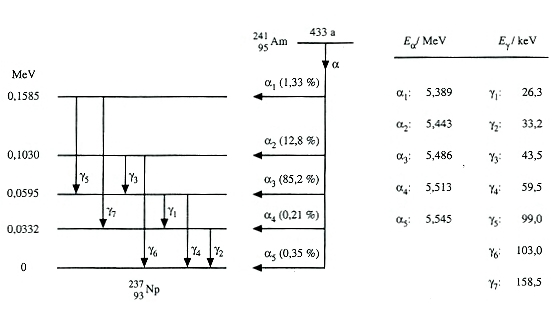
\includegraphics[width=0.9\linewidth]{6362cb7a8529daf05d8e0be425b50d10bacfe0c3}
	\caption{Zerfallsschema des Americium-Präparates, \cite{AmericiumZerfall}.}
	\label{fig:6362cb7a8529daf05d8e0be425b50d10bacfe0c3}
\end{figure}
\subsubsection{Annahmen zur Herleitung der Bethe-Bloch-Gleichung und der Rutherfordschen Streuformel}
Für die Herleitung der Bethe-Bloch-Gleichung wird angenommen, dass das schwere Teilchen eine Ruhemasse $m_0$ besitzt, die deutlich größer ist als die Ruhemasse eines Elektrons ($m_0 \gg m_e$). Eine Ablenkung bei der Wechselwirkung kommt also in diesem Fall nicht in Frage. Es wird angenommen, dass das Hüllenelektron sich vor der Wechselwirkung in Ruhe befindet und dieses frei ist.

Für die Rutherfordschen Streuformel wird angenommen, dass das Atom einen positiv geladenen Kern hat und dass sich um den Kern die negative Elementarladungen, Elektronen, mit verschwindend kleiner Masse befinden. Während der Streuung wird der Kern als ruhend angenommen, weil dieser eine höhere Masse als das $\alpha$-Teilchen besitzt. Als letztes wird noch angenommen, dass keine Mehrfachstreuung auftritt.

\subsubsection{Bestimmung des Bremsvermögens in Luft für die Alpha-Teilchen}
Trockene Luft besteht hauptsächlich aus rund $\SI{78,08}{\percent}$ Stickstoff und $\SI{20,95}{\percent}$ Sauerstoff. Mithilfe der Ionisationsenergien der beiden Stoffe sowie Ordnungs- und Massenzahlen wird mittels eine Mittelwertrechnung für Luft die folgenden Werte 
(s.Tabelle \ref{tab:datenluft}) berechnet:

\begin{table}[htpb]
	\centering
	\caption{Die Bestandteile aus Luft und die Mittelwertrechnung, \cite{Sauerstoff} \cite{Stickstoff} \cite{Sauerstoff0} \cite{Stickstoff0}.}
	\label{tab:datenluft}
	\begin{tabular}{r|r|r|r}
		\toprule
		Stoff	&	Ordnungszahl / Z &	Massenzahl / A &  Ionisationsenergie $/ \si{\electronvolt}$\\
		\hline
		Sauerstoff & 	8 & 16 & 95 \\
		Stickstoff &	7 & 14 & 82 \\
		Luft & 	7,5 & 15 & 88,5 \\
		\bottomrule
	\end{tabular}
\end{table}

Unter den Standardbedingungen (T = $\SI{298,15}{\kelvin}$)\cite{Luftdichte} beträgt die Luftdichte den folgenden Wert:
\begin{equation}
\rho = \SI{1,184}{\kilogram\per\cubic\meter}
\end{equation}
Damit kann das Bremsvermögen von $\alpha$-Teilchen in Luft berechnet werden und beträgt:
\begin{equation*}
-\frac{dE}{dx} = \SI{22,2815}{\frac{\mega\electronvolt}{\meter}}
\end{equation*}
Mit dem allgemeinen Gasgesetz kann anschließend der Luftdruck ermittelt werden:
\begin{equation}
p = \frac{\rho R T}{M}
\end{equation}
wobei $R$ die allgemeine Gaskonstante, $T$ die Temperatur unter den Standardbedingungen $\SI{298,15}{\kelvin}$ und $M$ die Molare Masse sind. Mit der Gleichung \ref{eq:bethebloch} wird für eine Wegstrecke von $\SI{100}{\milli\meter}$ ein Luftdruck von $\SI{12,19}{\pascal}$ berechnet.